\section{Analysis}
\subsection{speedup}
\subsection{image errors verification}
Since we made several changes in the algorithm where we introduced some slight innaccuracies (for example using a fixed-point representation instead of floating point in the DSP), errors are to be expected. Large errors are obvious to the eye, but this might be less obvious if the errors are only small. In this chapter we will detect and quantify these errors, to ensure that our implementation can still be considered correct.

\subsubsection{Error visualization}
Visualizing our errors is a fairly straightforward process. Because both images are constructed out of pixels with a grayscale value from 0 (black) to 255 (white), we can construct a new image by taking the difference between each pixel as a new pixel value. Note that this would give us a mapping where black indicates no difference, and brighter pixels indicating the difference. The inverse has more visual pop-out, so we subtract the difference from 255 to obtain our final pixel value. The implementation is described in Algorithm \ref{alg:imgdiff}. The result of this algorithm and a further comparison between the baseline and our implementation can be seen in figure~\ref{fig:imgdiff}.

\begin{algorithm}[t]
    \caption{Constructing a image with the differences between two images}\label{alg:imgdiff}
    \begin{algorithmic}[1]
        \Procedure{DiffImage}{$A[N],B[N]$}  \Comment{Images A and B both have a size of N pixels}
        \State $C[N]\gets 0$
        \For{$i\gets 0, n$}
           \State $C[i]\gets 255 - |A[i] - B[i]|$   \Comment{Subtract the difference of A and B from 255}
        \EndFor
        \State \textbf{return} $C$
        \EndProcedure
    \end{algorithmic}
\end{algorithm}

\begin{figure}
    \centering
    \begin{subfigure}[b]{0.3\textwidth}
                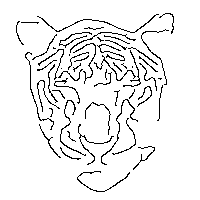
\includegraphics[width=\textwidth]{images/tiger_baseline}
                \caption{The baseline result}
                \label{fig:tiger_baseline}
        \end{subfigure}
        \begin{subfigure}[b]{0.3\textwidth}
                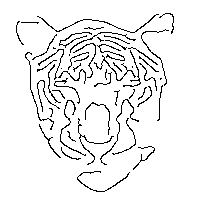
\includegraphics[width=\textwidth]{images/tiger_out}
                \caption{The optimized result}
                \label{fig:tiger_out}
        \end{subfigure}
        \begin{subfigure}[b]{0.3\textwidth}
                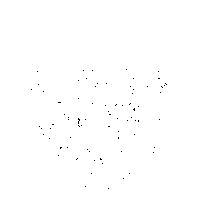
\includegraphics[width=\textwidth]{images/tiger_diff}
                \caption{The output of Algorithm~\ref{alg:imgdiff}}
                \label{fig:tiger_diff}
        \end{subfigure}
        \caption{Using the error visualization on an image of a tiger}\label{fig:imgdiff}
\end{figure}